
\subsection{Iteración 2}

Es necesario incorporar un avatar que represente las manos del jugador, así como añadir las posibles interacciones que este pueda realizar: coger, soltar, lanzar y cambiar de mano.

El plugin de SteamVR ya proporciona un avatar para las manos del jugador, así como para los mandos (figura \ref{fig:manos}), por lo que de momento se utilizarán esos recursos. 

\begin{figure}
  \centering
    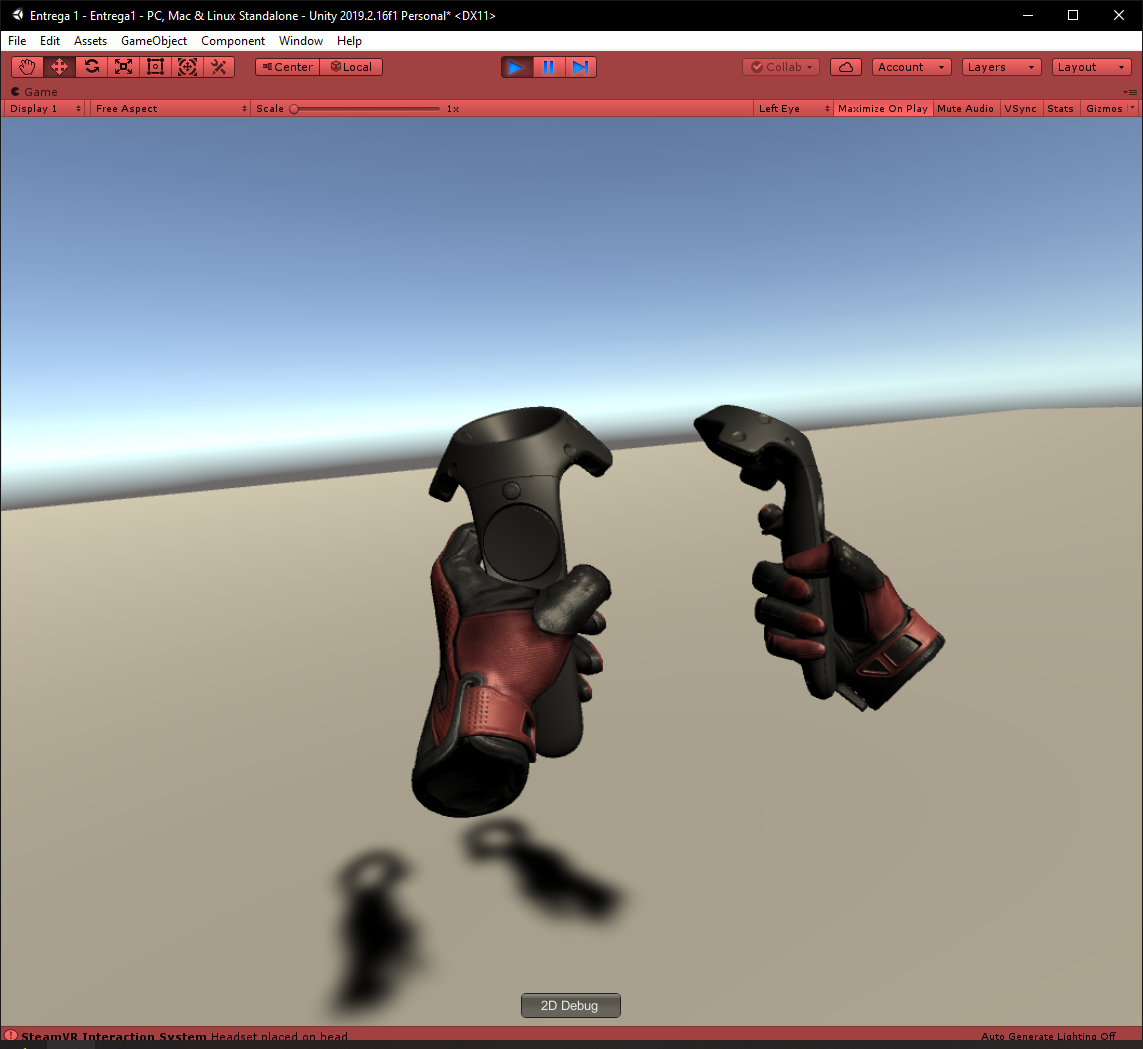
\includegraphics[width=0.7\textwidth]{04.Desarrollo/01.Entrega1/02.Iteracion1_2/00.Figuras/01.manos.png}
    \caption{Avatar por defecto de SteamVR.}
    \label{fig:manos}
\end{figure}


La mayoría de las interacciones estarán gestionadas por VRTK, por lo que a continuación se va a crear la estructura que enlaza el objeto del jugador de SteamVR con los sistemas de VRTK. Esto permite una mayor diversidad de interacciones y compatibilidad con otros dispositivos de realidad virtual que no están soportados por SteamVR mediante la capa de abstracción de VRTK.

El primer paso es hacer que VRTK gestione el movimiento de la cámara y los mandos, para ello al objeto ‘Player’ de la escena se le añade y enlaza el script de VRTK ‘Linked Alias Association Collection’ (figura \ref{fig:linkedAliasAssociationCollection}). Este script es el encargado de recoger los datos de los mandos y el visor de RV y pasárselos a VRTK.

\begin{figure}
  \centering
    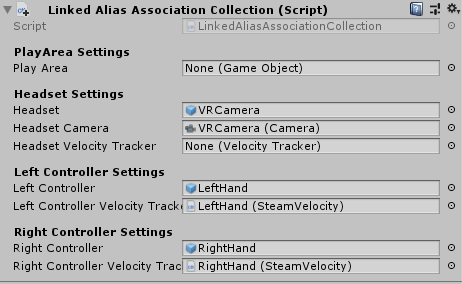
\includegraphics[width=0.6\textwidth]{04.Desarrollo/01.Entrega1/02.Iteracion1_2/00.Figuras/02.linked_alias_collection.png}
    \caption{Script ‘Linked Alias Association Collection’ enlazado con los objetos que representan las manos y la cabeza.}
    \label{fig:linkedAliasAssociationCollection}
\end{figure}

A continuación, se crea un sencillo script (figura \ref{fig:scriptVelocities}) cuyo objetivo es obtener la velocidad de un mando de SteamVR y devolverla en un formato adecuado para VRTK. Este script se añade a los objetos que representan las manos del jugador y se enlazan con el script de la sección anterior.

\begin{figure}
  \centering
    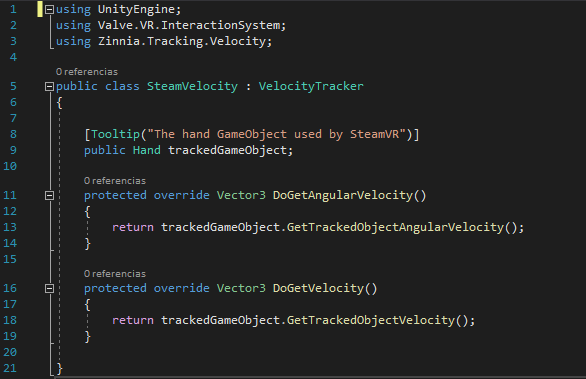
\includegraphics[width=0.6\textwidth]{04.Desarrollo/01.Entrega1/02.Iteracion1_2/00.Figuras/03.script_velocities.png}
    \caption{Script para obtener las velocidades de un objeto de SteamVR.}
    \label{fig:scriptVelocities}
\end{figure}

Por último, se crea un objeto que sea capaz de recoger y utilizar los datos que el objeto ‘Player’ está enviando. Para ello se utiliza un prefab de VRTK: TrackedAlias. Este objeto puede recibir información de varios ‘Player’ provenientes de distintos paquetes de RV, en este caso, de SteamVR. Véase figura \ref{fig:trackedAlias}.

\begin{figure}
  \centering
    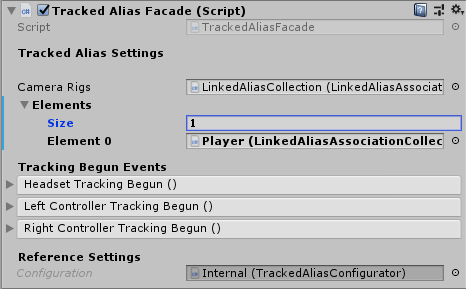
\includegraphics[width=0.6\textwidth]{04.Desarrollo/01.Entrega1/02.Iteracion1_2/00.Figuras/04.tracked_alias.png}
    \caption{TrackedAlias enlazado con el objeto Player.}
    \label{fig:trackedAlias}
\end{figure}


El segundo paso consiste en hacer que las acciones del jugados en los mandos (pulsaciones de botones) sean trasladadas a VRTK, para ello se utiliza el gestor de acciones nativo de Unity junto con un nuevo script (figura \ref{fig:scriptInput}) que recoge una acción de SteamVR y activa o desactiva una acción de Unity.

\begin{figure}
  \centering
    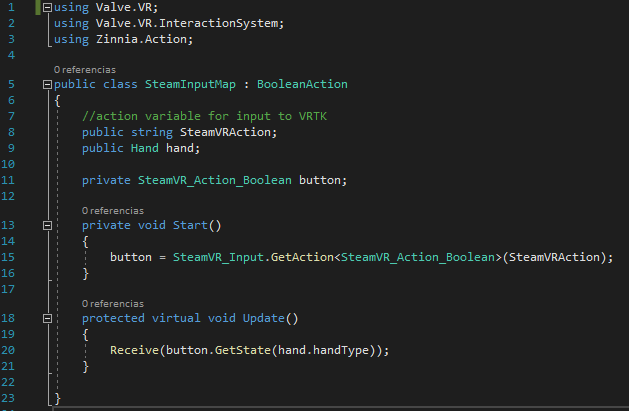
\includegraphics[width=0.6\textwidth]{04.Desarrollo/01.Entrega1/02.Iteracion1_2/00.Figuras/05.steam_input_map.png}
    \caption{Script para el manejo de acciones.}
    \label{fig:scriptInput}
\end{figure}

Este nuevo script debe estar asociado a un objeto del juego, por lo que hay que crear dos GameObject vacíos que contendrán los manejadores con el script (figura \ref{fig:handlers}), los cuales gestionarán las acciones generadas por cada uno de los dos mandos.

\begin{figure}
  \centering
    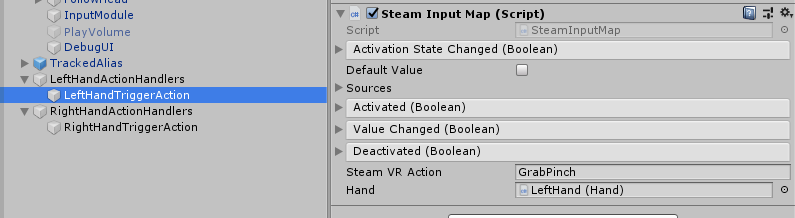
\includegraphics[width=0.8\textwidth]{04.Desarrollo/01.Entrega1/02.Iteracion1_2/00.Figuras/06.handlers.png}
    \caption{Manejadores para la acción de agarrar, activada por el gatillo del mando.}
    \label{fig:handlers}
\end{figure}

El último paso es añadir el objeto que proporciona VRTK para gestionar las interacciones de los mandos cuando utilizan las acciones manejadas en el paso anterior. Para ello se utiliza el prefab ‘Interactor’ y se anida dentro del objeto TrackedAlias, en concreto dentro de los alias de cada mando. Véase figura \ref{fig:interactorAnidado}.

\begin{figure}
  \centering
    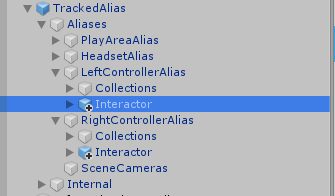
\includegraphics[width=0.5\textwidth]{04.Desarrollo/01.Entrega1/02.Iteracion1_2/00.Figuras/07.interactor_anidado.png}
    \caption{Interactors anidados en el objeto TrackedAlias.}
    \label{fig:interactorAnidado}
\end{figure}

Este ‘Interactor’ tiene un script llamado ‘Interactor Facade’ con un parámetro que permite definir cual será la acción de agarrar un objeto. Así que se utiliza el manejador creado anteriormente (figura \ref{fig:interactor}). 

\begin{figure}
  \centering
    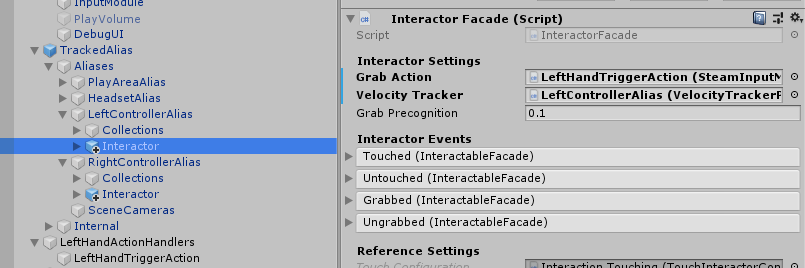
\includegraphics[width=0.8\textwidth]{04.Desarrollo/01.Entrega1/02.Iteracion1_2/00.Figuras/08.interactor.png}
    \caption{Interactor Facade con el manejador de acción definido anteriormente.}
    \label{fig:interactor}
\end{figure}

Finalmente es necesario añadir algún objeto con el que el jugador pueda interactuar. Para ello basta con crear un objeto 3D en la escena y añadirle los siguientes componentes (figura \ref{fig:interactable}):



\begin{itemize}
	\item{RigidBody: permite que el objeto actúe regido por las físicas del juego.}

	\item{Interactable: Script que permite que un objeto sea interactivo en RV.}
	
	\item{Velocity Estimator: Puede estimar la velocidad de un objeto cuando el jugador lo suelta.}
	
	\item{Throwable: Hace que el jugador pueda lanzar el objeto.}
	
	\item{Steam VR Skeleton Poser: Permite definir la pose que adoptará la mano del jugador al interactuar con el objeto.}

\end{itemize}

\begin{figure}
  \centering
    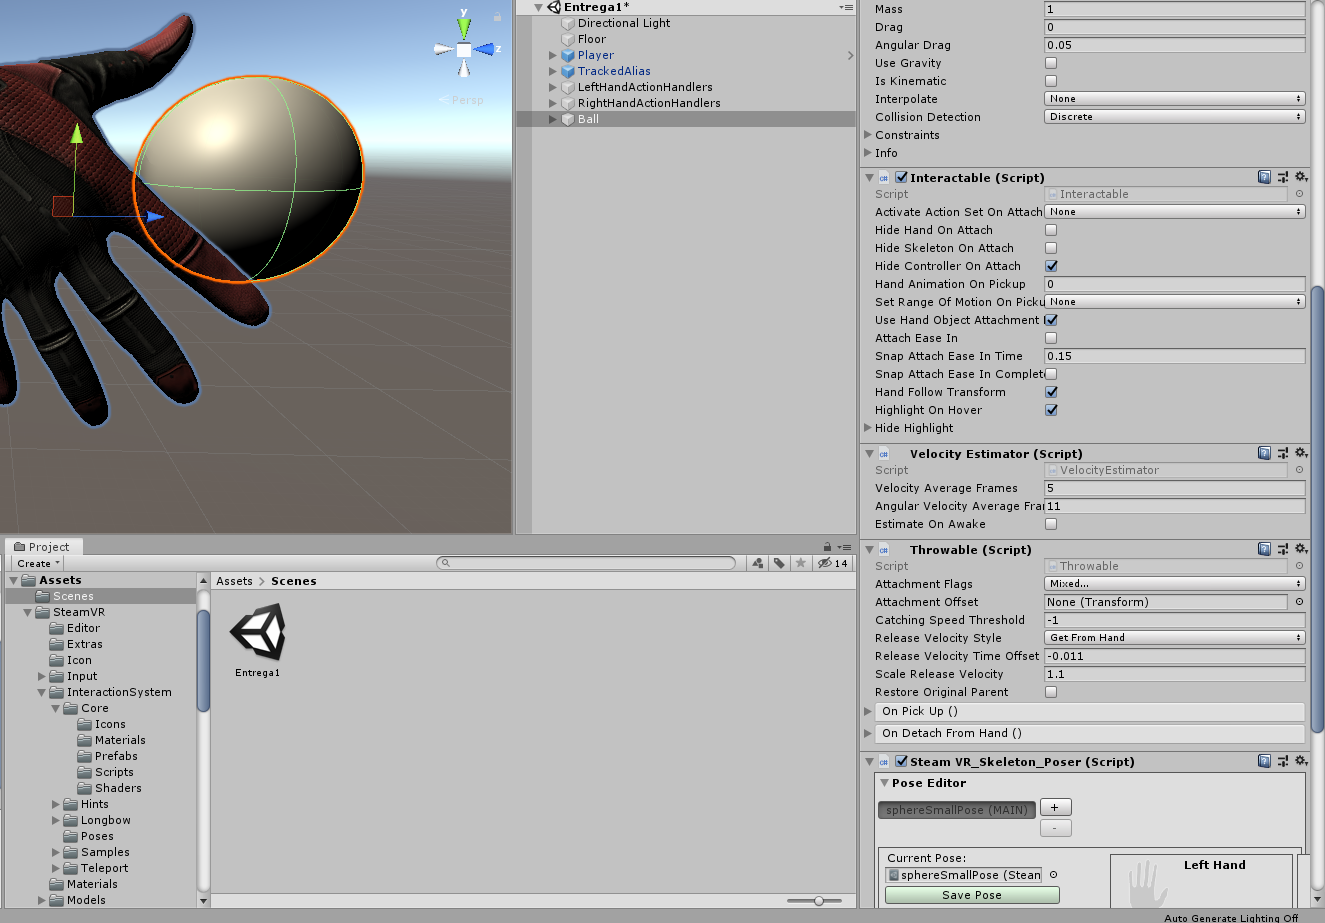
\includegraphics[width=0.9\textwidth]{04.Desarrollo/01.Entrega1/02.Iteracion1_2/00.Figuras/09.bola.png}
    \caption{Objeto interactivo con los componentes necesarios para la RV.}
    \label{fig:interactable}
\end{figure}

Con estos pasos terminados, el proyecto cuenta ya con un entorno en realidad virtual con todas las funcionalidades de SteamVR y VRTK. En este entorno el jugador puede coger objetos con sus manos, soltarlos, lanzarlos o cambiarlos de mano fácilmente (figura \ref{fig:esferaCogida}).


\begin{figure}
  \centering
    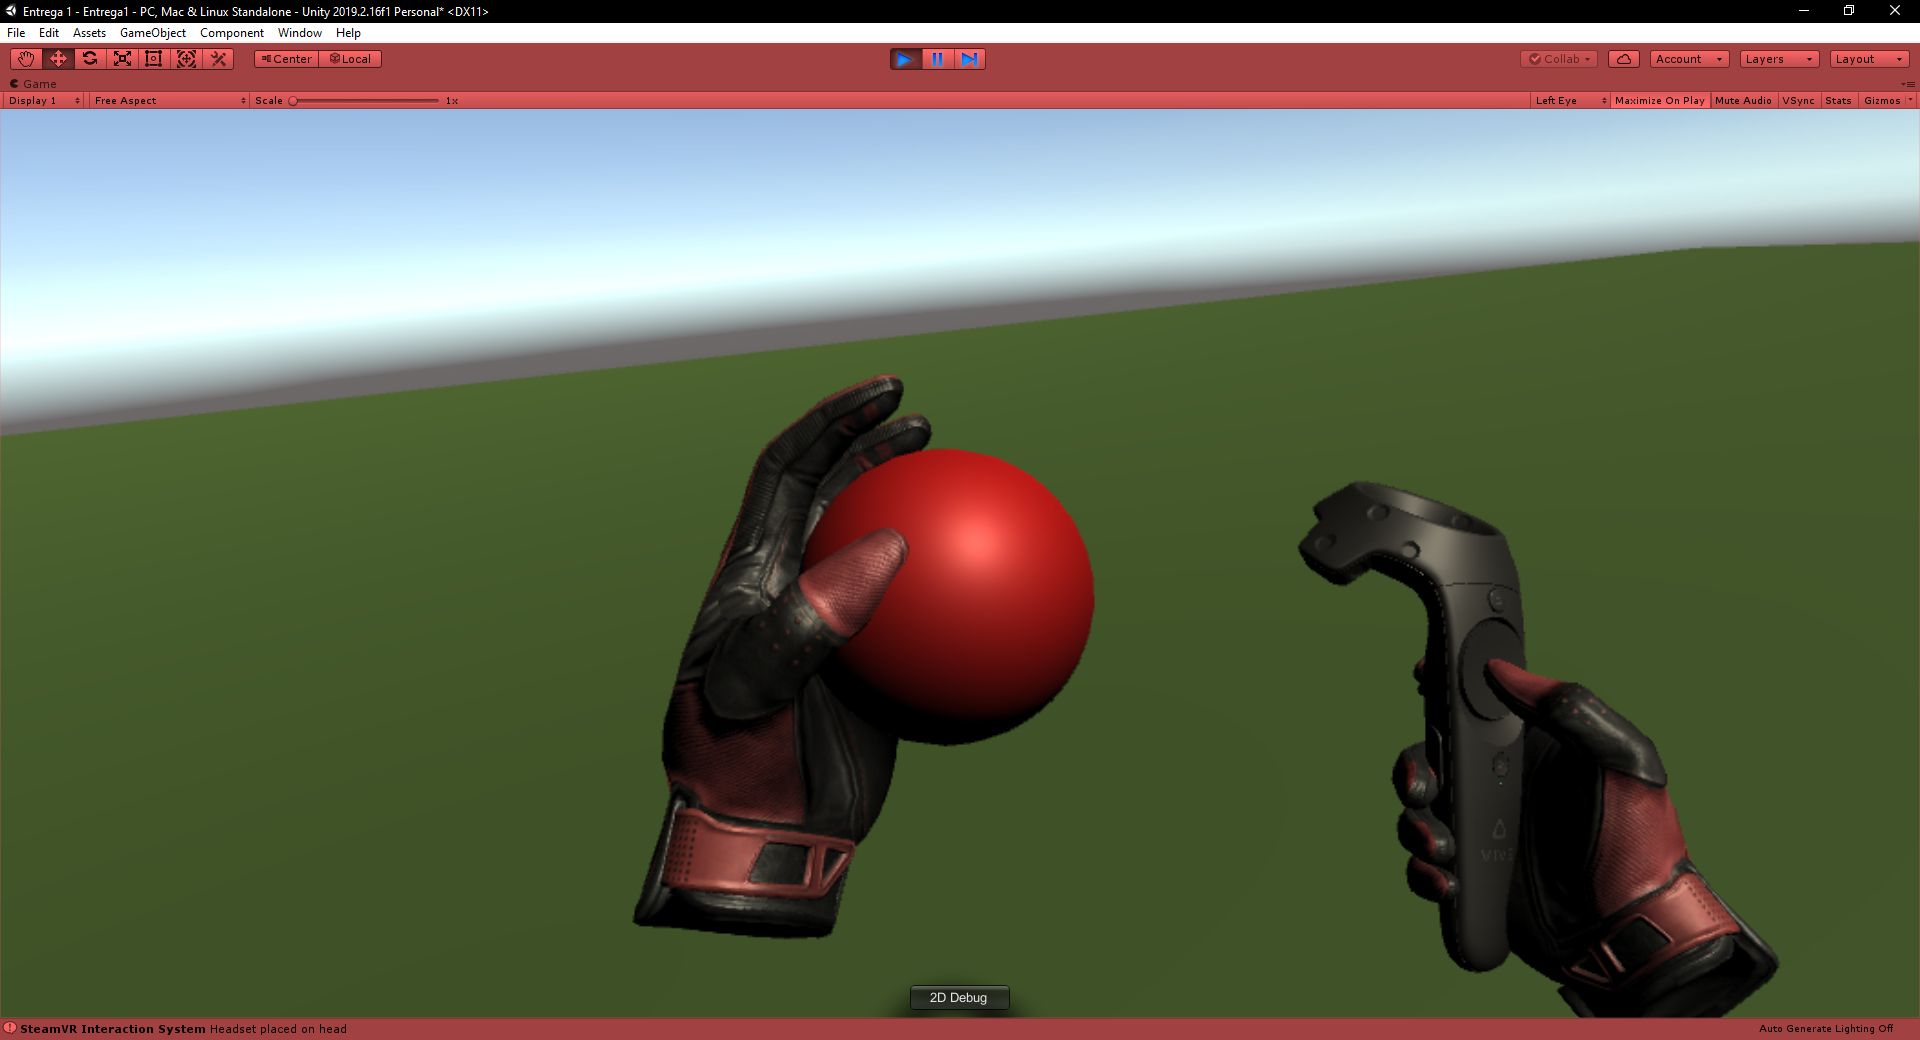
\includegraphics[width=0.9\textwidth]{04.Desarrollo/01.Entrega1/02.Iteracion1_2/00.Figuras/10.manos_2.png}
    \caption{Avatar cogiendo una esfera interactiva.}
    \label{fig:esferaCogida}
\end{figure}


